\section{Paper Formatting}

Please read this tex file carefully to learn about the paper submission format. This section is to be deleted for your submission.

\subsection{Paper length}

The length requirements for the project outline and the final project report are different. Please read the instructions on the website carefully.

\subsection{Layout, Typeface, Font Sizes, and Numbering}

The paper format setup is usually included in the latex templates you download from a journal or conference website. An incorrect format can lead to a rejection.

Typically, all lines should be numbered in a manuscript submission for the efficiency of paper review. In a camera-ready version, line numbering is usually not preferred. To learn about the submission format requirements, it is crucial to read the instructions carefully. For your final project, we accept either format.

\subsection{Sections}

The five sections in this file provides you a starting point. You do not need to go with this format, but keep in mind that a detailed paper should include an introduction, a related work/background survey, methods and experiments, and conclusions.

\subsection{Citations}

For the papers you'd like to cite, you can go to Google Scholar and search for the paper. Click on the button "cite" on the Google Scholar page, and select "BibTex". This is bring you to the BibTex page. You can copy the texts and paste them to your bibliography file, such as "egbib.bib". You may use this file or create you own. If latter, you will need to change the file name in main.tex. In your paper, you can use the following method to call on the bibliography numbering: Visual Question Answering~\cite{antol2015vqa} introduces the VQA task.

\subsection{Basic Functions and Structuring Tools}

Below are some commonly used formatting skills that might be helpful for structuring your paper. For more details, you can visit the Overleaf tutorial: \url{https://www.overleaf.com/learn/latex/Tutorials}

\subsubsection{Mathematics}

Please number all of your sections and displayed equations.  Again,
this makes reviewing more efficient, because reviewers can refer to a line on a page.  Also, it is important for readers to be able to refer to any particular equation.  Just because you didn't refer to it in the text doesn't mean some future reader might not need to refer to it.  It is cumbersome to have to use circumlocutions like ``the equation second from the top of page 3 column 1''.  (Note that the line numbering will not be present in the final copy, so is not an alternative to equation numbers).

\subsubsection{Headings.}

Headings should be capitalized (i.e., nouns, verbs, and all other words except articles, prepositions, and conjunctions should be set with an initial capital) and should,
with the exception of the title, be aligned to the left.
Words joined by a hyphen are subject to a special rule. If the first word can stand alone, the second word should be capitalized.
The font sizes are given in Table~\ref{table:headings}.

\setlength{\tabcolsep}{4pt}

\begin{table}
\begin{center}
\caption{Font sizes of headings. Table captions should always be
positioned {\it above} the tables. The final sentence of a table
caption should end without a full stop}
\label{table:headings}
\begin{tabular}{lll}
\hline\noalign{\smallskip}
Heading level & Example & Font size and style\\
\noalign{\smallskip}
\hline
\noalign{\smallskip}
Title (centered)  & {\Large \bf Lecture Notes \dots} & 14 point, bold\\
1st-level heading & {\large \bf 1 Introduction} & 12 point, bold\\
2nd-level heading & {\bf 2.1 Printing Area} & 10 point, bold\\
3rd-level heading & {\bf Headings.} Text follows \dots & 10 point, bold
\\
4th-level heading & {\it Remark.} Text follows \dots & 10 point,
italic\\
\hline
\end{tabular}
\end{center}
\end{table}
\setlength{\tabcolsep}{1.4pt}

Here are some examples of headings: ``Criteria to Disprove Context-Freeness of Collage Languages'', ``On Correcting the Intrusion of Tracing Non-deterministic Programs by Software'', ``A User-Friendly and Extendable Data Distribution System'', ``Multi-flip Networks: Parallelizing GenSAT'', ``Self-determinations of Man''.

\subsubsection{Lemmas, Propositions, and Theorems.}

The numbers accorded to lemmas, propositions, and theorems etc. should appear in consecutive order, starting with the number 1, and not, for example, with the number 11.

\subsubsection{Figures and Photographs}
\label{sect:figures}

Please produce your figures electronically and integrate
them into your text file. For \LaTeX\ users we recommend using package \verb+graphicx+ or the style files \verb+psfig+ or \verb+epsf+.

Check that in line drawings, lines are not interrupted and have constant width. Grids and details within the figures must be clearly readable and may not be written one on top of
the other. Line drawings should have a resolution of at least 800 dpi (preferably 1200 dpi).
For digital halftones 300 dpi is usually sufficient.
The lettering in figures should have a height of 2~mm (10-point type). Figures should be scaled up or down accordingly.
Please do not use any absolute coordinates in figures.

Figures should be numbered and should have a caption which should
always be positioned {\it under} the figures, in contrast to the caption belonging to a table, which should always appear {\it above} the table. Please center the captions between the margins and set them in 9-point type (Fig.~\ref{fig:example} shows an example). The distance between text and figure should be about 8~mm, the distance between figure and caption about 5~mm.
\begin{figure}
\centering
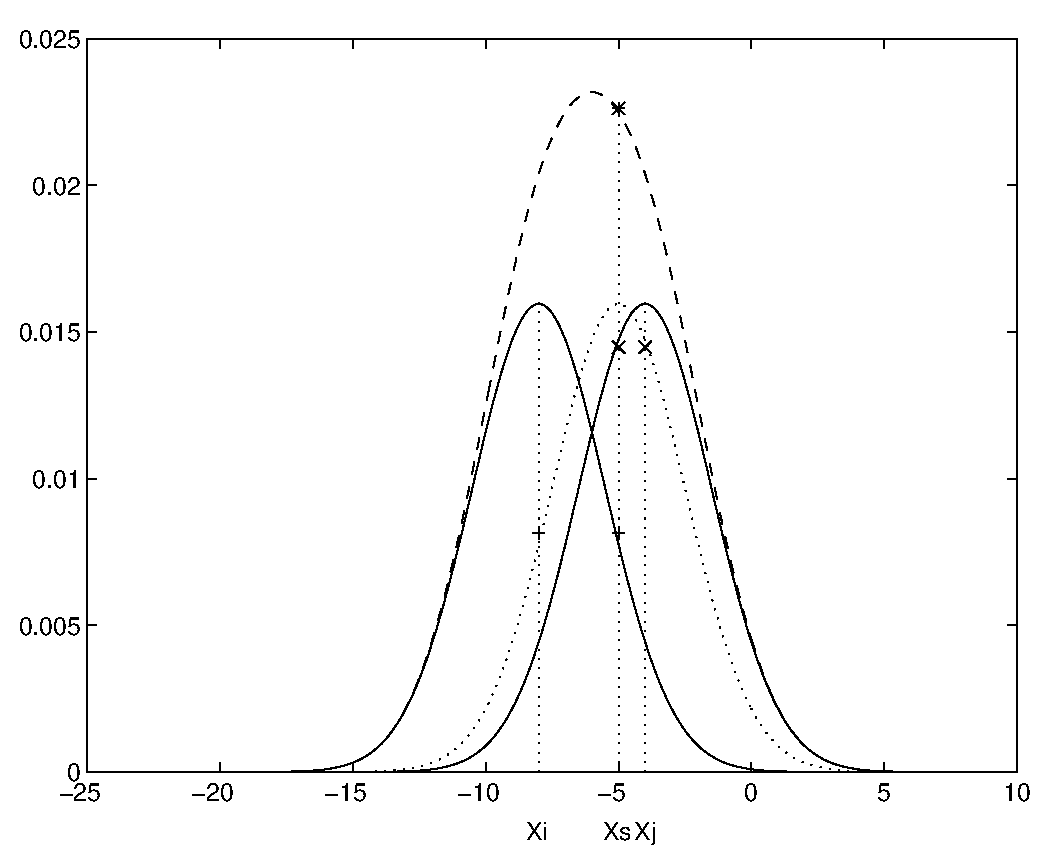
\includegraphics[height=6.5cm]{images/eijkel2}
\caption{One kernel at $x_s$ ({\it dotted kernel}) or two kernels at $x_i$ and $x_j$ ({\it left and right}) lead to the same summed estimate at $x_s$. This shows a figure consisting of different types of lines. Elements of the figure described in the caption should be set in italics, in parentheses, as shown in this sample caption. The last sentence of a figure caption should generally end without a full stop}
\label{fig:example}
\end{figure}

If possible (e.g. if you use \LaTeX) please define figures as floating objects. \LaTeX\ users, please avoid using the location
parameter ``h'' for ``here''. If you have to insert a pagebreak before a figure, please ensure that the previous page is completely filled.

\subsubsection{Formulas}

Displayed equations or formulas are centered and set on a separate
line (with an extra line or halfline space above and below). Displayed expressions should be numbered for reference. The numbers should be consecutive within the contribution,
with numbers enclosed in parentheses and set on the right margin.
For example,
\begin{align}
  \psi (u) & = \int_{0}^{T} \left[\frac{1}{2}
  \left(\Lambda_{0}^{-1} u,u\right) + N^{\ast} (-u)\right] dt \; \\
& = 0 ?
\end{align}

Please punctuate a displayed equation in the same way as ordinary
text but with a small space before the end punctuation.

\subsubsection{Footnotes}

The superscript numeral used to refer to a footnote appears in the text either directly after the word to be discussed or, in relation to a phrase or a sentence, following the punctuation sign (comma, semicolon, or full stop). Footnotes should appear at the bottom of the normal text area, with a line of about 2~cm in \TeX\ and about 5~cm in Word set immediately above them.\footnote{The footnote numeral is set flush left and the text follows with the usual word spacing. Second and subsequent lines are indented. Footnotes should end with a full stop.}


\subsubsection{Program Code}

Program listings or program commands in the text are normally set in typewriter font, e.g., CMTT10 or Courier.

\noindent
{\it Example of a Computer Program}
\begin{verbatim}
program Inflation (Output)
  {Assuming annual inflation rates of 7%, 8%, and 10%,...
   years};
   const
     MaxYears = 10;
   var
     Year: 0..MaxYears;
     Factor1, Factor2, Factor3: Real;
   begin
     Year := 0;
     Factor1 := 1.0; Factor2 := 1.0; Factor3 := 1.0;
     WriteLn('Year  7% 8% 10%'); WriteLn;
     repeat
       Year := Year + 1;
       Factor1 := Factor1 * 1.07;
       Factor2 := Factor2 * 1.08;
       Factor3 := Factor3 * 1.10;
       WriteLn(Year:5,Factor1:7:3,Factor2:7:3,Factor3:7:3)
     until Year = MaxYears
end.
\end{verbatim}
%
\noindent
{\small (Example from Jensen K., Wirth N. (1991) Pascal user manual and
report. Springer, New York)}

